\definecolor{lightgray}{gray}{0.95}

\newcommand{\risultati}[4]{
  \subsubsection{Results}
  This model achieved the following results at the end of training:
  \begin{table}[H]
  \centering
  \rowcolors{2}{lightgray}{white}
  \begin{tabular}{@{} >{\bfseries}l c @{}}
    \toprule
    \textbf{Metric}    & \textbf{Value} \\
    \midrule
    Loss                & #1              \\
    Validation Loss     & #2              \\
    Accuracy            & #3              \\
    Validation Accuracy & #4              \\
    \bottomrule
  \end{tabular}
  \caption{Results of the model at the end of training}
  \label{tab:risultati}
  \end{table}
}

\newcommand{\training}[8]{
  \subsubsection{Training}
  The training of the model was carried out using the following configuration:
  \begin{table}[ht]
    \centering
    \rowcolors{2}{lightgray}{white}
    \begin{tabular}{@{} >{\bfseries}l c @{}}
      \toprule
      \textbf{Parameter}        & \textbf{Value} \\
      \midrule
      Optimizer                 & #1              \\
      Learning rate             & #2              \\
      Embedding dimension       & #3              \\
      Latent dimension          & #4              \\
      Decoder dropout           & #5              \\
      Decoder recurrent dropout & #6              \\
      Encoder dropout           & #7              \\
      Encoder recurrent dropout & #8              \\
      \trainingcontinued
      }

      \newcommand{\trainingcontinued}[2]{
      Batch size                & #1              \\
      Epochs                    & #2              \\
      \bottomrule
    \end{tabular}
    \caption{Training configuration}
  \end{table}

  \lossimg
}

\newcommand{\lossimg}[2]{
  We can check the trend of the losses during training in Figure \ref{fig:#2}.

  \begin{figure}[H]
    \centering
    \includegraphics[width=0.75\textwidth]{media/#1_best_lossplot.png}
    \caption{Trend of the \textit{loss} and \textit{validation loss} during training}
    \label{fig:#2}

  \end{figure}
}

\newcommand{\architecture}[3]{
  \subsubsection{Architecture}
  The architecture used is as follows:
  \archimg{#1}{#2}{#3}
}

\newcommand{\archimg}[3]{
  \begin{figure}[H]
    \centering
    \includegraphics[width=0.75\textwidth]{media/#1_best_architecture.png}
    \caption{Architecture of the model #2}
    \label{fig:#3}
  \end{figure}
}

\newcommand{\rougeonesubimg}[3]{
  \begin{subfigure}{#1\textwidth}
    \centering
    \includegraphics[width=\textwidth]{media/#2_best_rouge1_scores.png}
    \caption{ROUGE-1 #2}
    \label{fig:#3}
  \end{subfigure}
}

\newcommand{\rougetwosubimg}[3]{
  \begin{subfigure}{#1\textwidth}
    \centering
    \includegraphics[width=\textwidth]{media/#2_best_rouge2_scores.png}
    \caption{ROUGE-2 #2}
    \label{fig:#3}
  \end{subfigure}
}

\newcommand{\rougelubimg}[3]{
  \begin{subfigure}{#1\textwidth}
    \centering
    \includegraphics[width=\textwidth]{media/#2_best_rougeL_scores.png}
    \caption{ROUGE-L #2}
    \label{fig:#3}
  \end{subfigure}
}

\newcommand{\wersubimg}[3]{
  \begin{subfigure}{#1\textwidth}
    \centering
    \includegraphics[width=\textwidth]{media/#2_best_wer_scores.png}
    \caption{WER #2}
    \label{fig:#3}
  \end{subfigure}
}

\newcommand{\cssubimg}[3]{
  \begin{subfigure}{#1\textwidth}
    \centering
    \includegraphics[width=\textwidth]{media/#2_best_cosine_similarity_scores.png}
    \caption{Cosine similarity #2}
    \label{fig:#3}
  \end{subfigure}
}

\newcommand{\bertsubimg}[3]{
  \begin{subfigure}{#1\textwidth}
    \centering
    \includegraphics[width=\textwidth]{media/#2_best_bert_scores.png}
    \caption{BERT score #2}
    \label{fig:#3}
  \end{subfigure}
}

\newcommand{\myevalsubimg}[3]{
  \begin{subfigure}{#1\textwidth}
    \centering
    \includegraphics[width=\textwidth]{media/#2_best_myevaluation_scores.png}
    \caption{My Evaluation #2}
    \label{fig:#3}
  \end{subfigure}
}

\section{Architettura dei Modelli}
L'implementazione dei modelli è stata effettuata attraverso una classe astratta \texttt{BaseModel} e la successiva creazioni e implementazione di classi derivate.\\
Questo permette di definire un'interfaccia comune per tutti i modelli di summarization e di estendere facilmente l'architettura in futuro.\\

\subsection{Classe Base Astratta}
La classe \texttt{BaseModel} fornisce l'interfaccia base per tutti i modelli di summarization:
\begin{itemize}
    \item Metodi astratti per costruire encoder e decoder.
    \item Funzionalità per il salvataggio, caricamento e inferenza del modello.
    \item Conversione tra sequenze e testo tramite i tokenizer.
\end{itemize}

\subsection{Training}
L'addestramento dei modelli, derivati dalla classe \texttt{BaseModel}, è stato effettuato utilizzando il dataset preprocessato.\\
Prima di iniziare l'addestramento, il dataset è stato suddiviso in training set e validation set, con una proporzione del 90\% e 10\% rispettivamente.\\
Dopodiché sono passato alla fase effettiva di training dei modelli, utilizzando e la loss function \texttt{Sparse Categorical Crossentropy}, utile nei task di summarization.\\

\subsubsection{Callbacks}
Durante il training ho utilizzato anche le seguenti funzioni di callback:
\begin{itemize}
    \item \textbf{Early Stopping}: monitora una metrica, in questo caso la validation loss, e interrompe l'addestramento se non ci sono miglioramenti per un certo numero di epoche consecutive. Questo aiuta a prevenire l'overfitting e a risparmiare tempo di calcolo.
    \item \textbf{Learning Rate Scheduler}: regola il tasso di apprendiento durante il training secondo una strategia, nel mio caso ho utilizzato la \texttt{Step Decay}, che riduce il learning rate di un fattore fisso ogni tot epoche.
    \item \textbf{Reduce LR on Plateau}: monitora una metrica, in questo caso la validation loss, e riduce il learning rate se non ci sono miglioramenti per un certo numero di epoche consecutive. Questo aiuta a ottimizzare il processo di addestramento e a trovare un tasso di apprendimento più efficace.
\end{itemize}

\subsection{Architetture sperimentate}
Sono state sperimentante diverse architetture di modelli di summarization, ognuna con caratteristiche e parametri diversi.\\
Le due categorie principali di modelli implementati sono:
\begin{itemize}
    \item \textbf{LSTM}: modelli basati su layer LSTM per encoder e decoder.
    \item \textbf{GRU}: modelli basati su layer GRU per encoder e decoder.
\end{itemize}
Tali architetture sono basate sulle RNN (Recurrent Neural Networks) e sono state scelte per la loro efficacia nei task di text-summarization, poiché 
gestiscono le dipendenze tra le parole su sequenze di testo.\\ 
\begin{itemize}
    \item \textbf{LSTM}: Long Short-Term Memory, è una variante delle RNN che risolve il problema del vanishing gradient, grazie alla presenza di un meccanismo di memoria a lungo termine.
    Tale meccanismo di gating permette di memorizzare informazioni importanti e scartare quelle meno rilevanti.
    \item \textbf{GRU}: Gated Recurrent Unit, è una variante più semplice delle LSTM, con meno parametri e meno complessità computazionale.
    Anche in questo caso, il meccanismo di gating permette di memorizzare informazioni importanti e scartare quelle meno rilevanti.
\end{itemize}

Al fine di rendere più scorrevole la lettura, per ogni classe vengono riportati solamente i migliori risultati ottenuti durante l'addestramento con i migliori parametri e le migliori configurazioni trovate, sebbene
siano stati effettuati numerosi tentativi e test riportati in seguito in una tabella comparativa.\\


\subsection{Seq2SeqLSTM}
The \texttt{Seq2SeqLSTM} class implements the specific architecture for the Sequence to Sequence summarization model with LSTM layers.

\training{Adam}{0.001}{512}{128}{0.2}{0.2}{0.2}{0.2}{128}{50}{Seq2SeqLSTM}{seq2seqlstm_loss_plot}
\risultati{1.63}{2.02}{0.67}{0.64}
\architecture{Seq2SeqLSTM}{Seq2SeqLSTM}{seq2seqlstm_architecture}

\subsection{Seq2SeqBiLSTM}
La classe \texttt{Seq2SeqBiLSTM} implementa un'architettura simile al modello Seq2SeqLSTM, ma i layer LSTM dell'encoder sono bidirezionali.

\training{Adam}{0.001}{512}{256}{0.2}{0.2}{0.2}{0.2}{64}{50}{Seq2SeqBiLSTM}{seq2seqbilstm_loss_plot}
\risultati{1.23}{2.01}{0.72}{0.65}
\architecture{Seq2SeqBiLSTM}{Seq2SeqBiLSTM}{seq2seqbilstm_architecture}
\subsection{Seq2Seq3BiLSTM}
The \texttt{Seq2Seq3BiLSTM} class implements an architecture similar to the Seq2SeqBiLSTM model, but with three bidirectional LSTM layers in the encoder.

\training{Adam}{0.001}{256}{256}{0.2}{0.2}{0.2}{0.2}{128}{50}{Seq2Seq3BiLSTM}{seq2seq3bilstm_loss_plot}
\risultati{1.51}{1.99}{0.68}{0.65}
\architecture{Seq2Seq3BiLSTM}{Seq2Seq3BiLSTM}{seq2seq3bilstm_architecture}
\subsection{Seq2SeqLSTMGloVe}
La classe \texttt{Seq2SeqLSTMGloVe} implementa un'architettura simile al modello Seq2SeqLSTM, utilizzando i vettori di embedding GloVe preaddestrati per la rappresentazione delle parole.\\
Più precisamente vengono scaricati e utilizzati i vettori di embedding GloVe preaddestrati da \href{https://nlp.stanford.edu/projects/glove/}{Stanford NLP Group} da 100 dimensioni, anche se la classe consente di scambiare facilmente i vettori con quelli di dimensione diversa.\\

\training{Adam}{50}
\risultati{DA INSERIRE}{DA INSERIRE}{DA INSERIRE}{DA INSERIRE}
Possiamo verifcare l'andamento delle loss durante l'addestramento nella figura \ref{fig:seq2seqlstmglove_loss_plot}.
\begin{figure}[H]
    \centering
    \includegraphics[width=0.75\textwidth]{media/Seq2SeqLSTMGloVe_originale_lossplot.png}
    \caption{Andamento delle loss durante l'addestramento}
    \label{fig:seq2seqlstmglove_loss_plot}
\end{figure}

%\subsection{Seq2SeqLSTMTrasformer}
La classe \texttt{Seq2SeqLSTMTrasformer} implementa un'architettura simile al modello Seq2SeqLSTM, ma inoltre aggiunge \(2\) blocchi Transformer sia nell'encoder che nel decoder.\\

\subsubsection{Encoder}
\begin{itemize}
    \item \textbf{Layer di embedding}
    \item \textbf{Due Blocchi Transformer} con:
        \begin{itemize}
            \item Dimensione latente pari a 300
            \item Dropout del 40\%
        \end{itemize}
    \item \textbf{Tre layer LSTM} con:
    \begin{itemize}
        \item Dimensione latente pari a 300
        \item Dropout del 40\%
        \item Recurrent dropout del 40\%
    \end{itemize}
\end{itemize}

\subsubsection{Decoder}
\begin{itemize}
    \item \textbf{Layer di embedding}
    \item \textbf{Due blocchi Transformer} con:
        \begin{itemize}
            \item Dimensione latente pari a 300
            \item Dropout del 40\%
            \item Recurrent dropout del 20\%
            \item Un MultiHeadAttention da \(8\) Head
            \item Un layer di Dropout del 10\%
            \item Un Add layer
            \item Un layer di Normalizzazione
            \item Tre layer di FeedForward con:
                \begin{itemize}
                    \item Un layer denso con attivazione ReLU e dimensione latente pari a \(512\)
                    \item Un layer denso con dimensione latente pari a \(300\)
                    \item Un layer di Dropout del 10\%
                    \item Un Add layer
                    \item Un layer di Normalizzazione
                \end{itemize}
        \end{itemize}
    \item \textbf{Layer LSTM} con:
        \begin{itemize}
            \item Stessa dimensione latente dell'encoder
            \item Dropout del 40\%
            \item Recurrent dropout del 40\%
        \end{itemize}
    \item \textbf{Layer di attention}
    \item \textbf{Layer denso di output}
\end{itemize}

Di seguito, possiamo vedere un diagramma dell'architettura del modello Seq2SeqLSTMTrasformer nella figura \ref{fig:seq2seqlstmtrasformer_model_architecture}.
\begin{figure}[H]
    \centering
    \includegraphics[width=0.55\textwidth]{media/Seq2SeqLSTMTransformer_image.png}
    \caption{Diagramma dell'architettura del modello Seq2SeqLSTMTrasformer}
    \label{fig:seq2seqlstmtrasformer_model_architecture}
\end{figure}

\training{Adam}{50}
\risultati{0.2015}{0.5034}{0.9576}{0.9269}

Possiamo verificare l'andamento della funzione di loss durante l'addestramento del modello nella figura \ref{fig:seq2seqlstmtrasformer_loss}.
\begin{figure}[H]
    \centering
    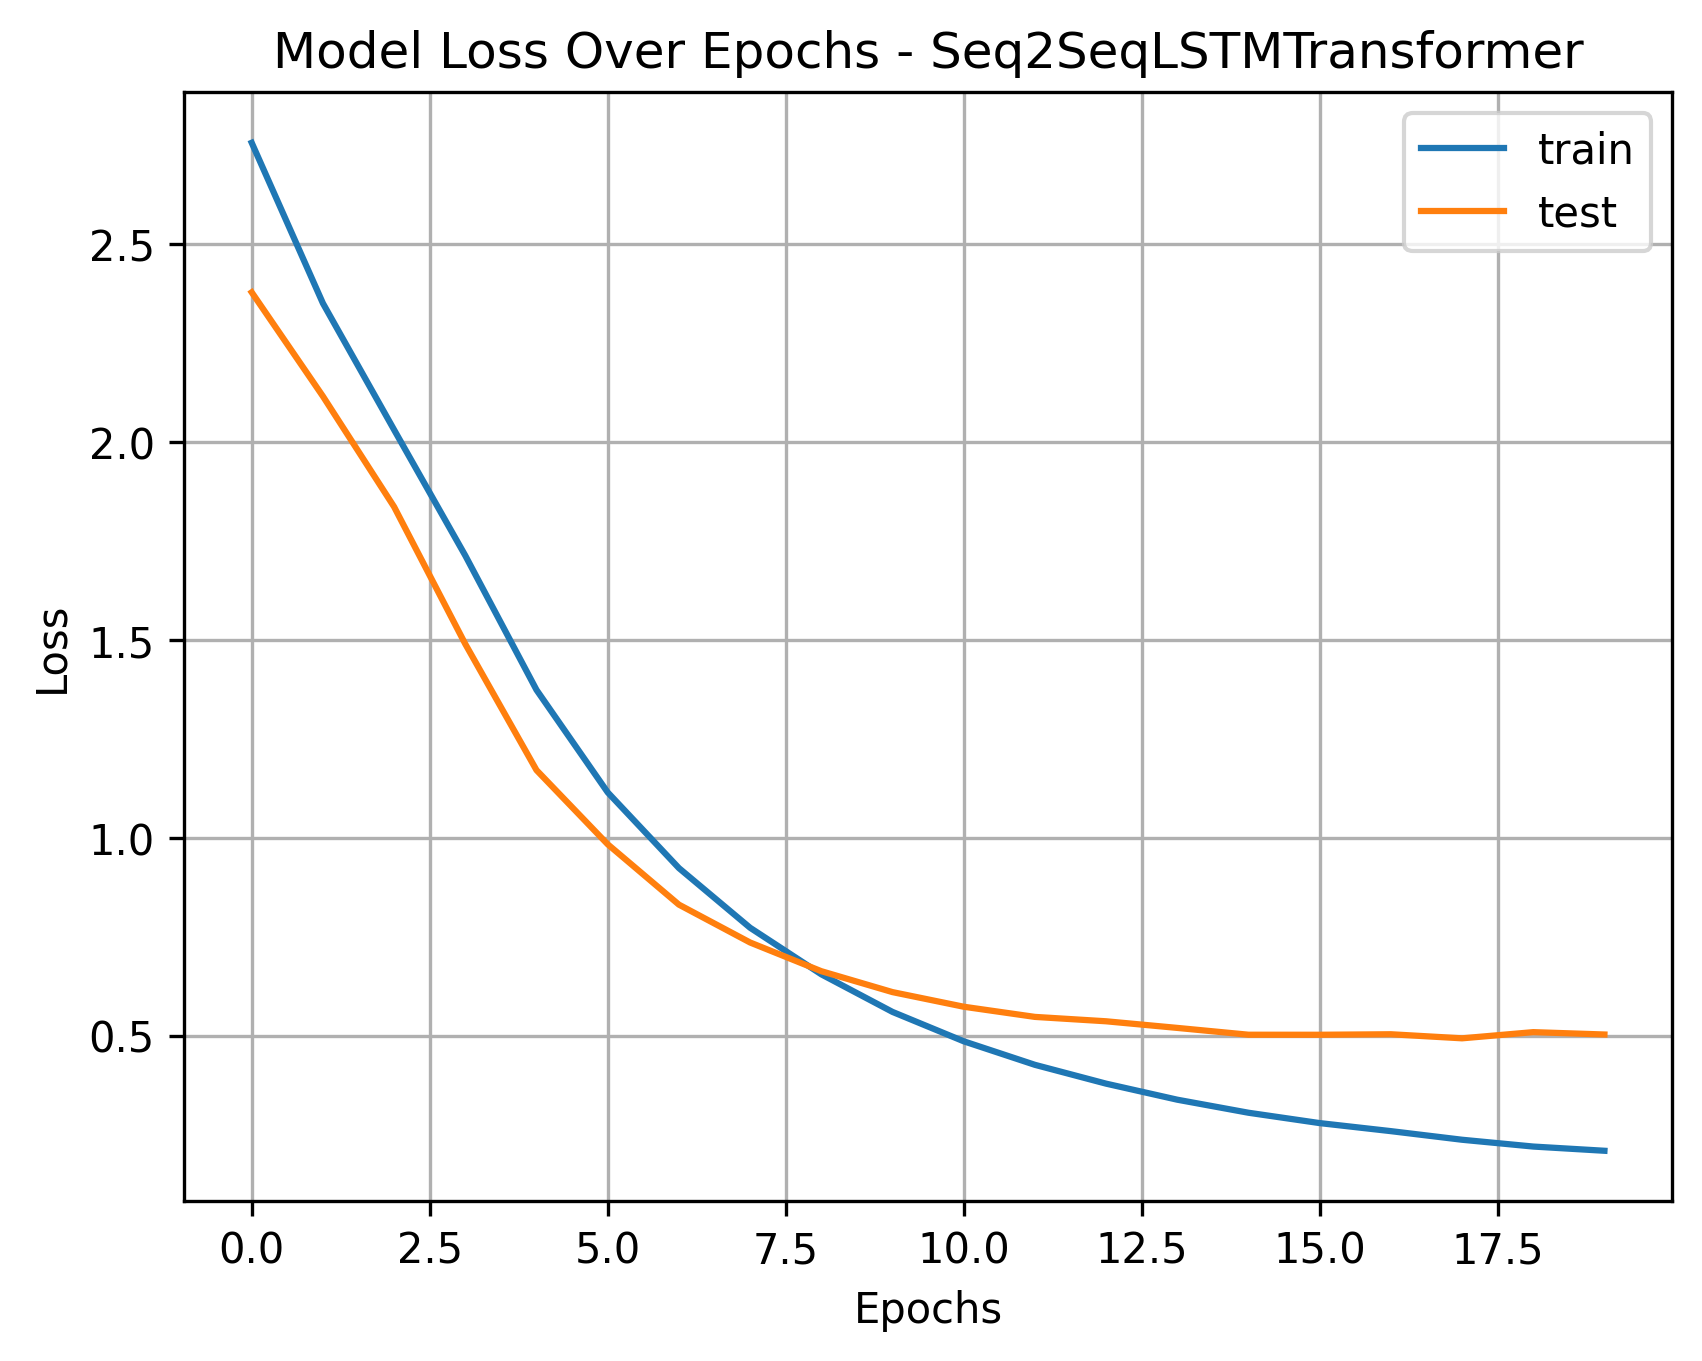
\includegraphics[width=0.65\textwidth]{media/Seq2SeqLSTMTransformer_originale_lossplot.png}
    \caption{Andamento della funzione di loss durante l'addestramento del modello Seq2SeqLSTMTrasformer}
    \label{fig:seq2seqlstmtrasformer_loss}
\end{figure}


\subsection{Confronto tra le Architetture}
\begin{figure}[H]
    \centering
    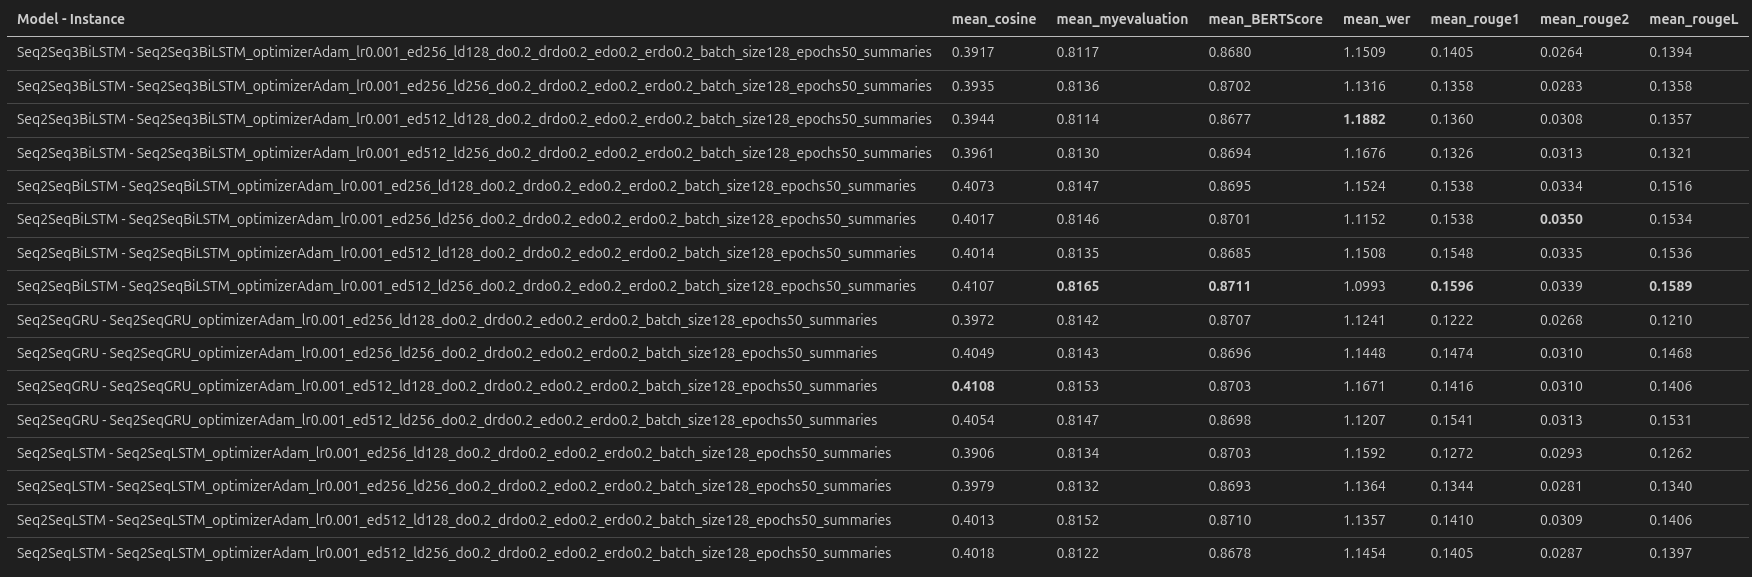
\includegraphics[width=1\textwidth]{media/models_comparison_instances.png}
    \caption{Comparazione delle istanze dei modelli}
    \label{fig:models_comparison_instances}
\end{figure}
  
